\documentclass[../../main]{subfiles}
\begin{document}
This semester project revolves around the control of a dynamic system, more specific a pan-tilt  system shown in figure \ref{fig:system}.

\begin{figure}[H]
\centering
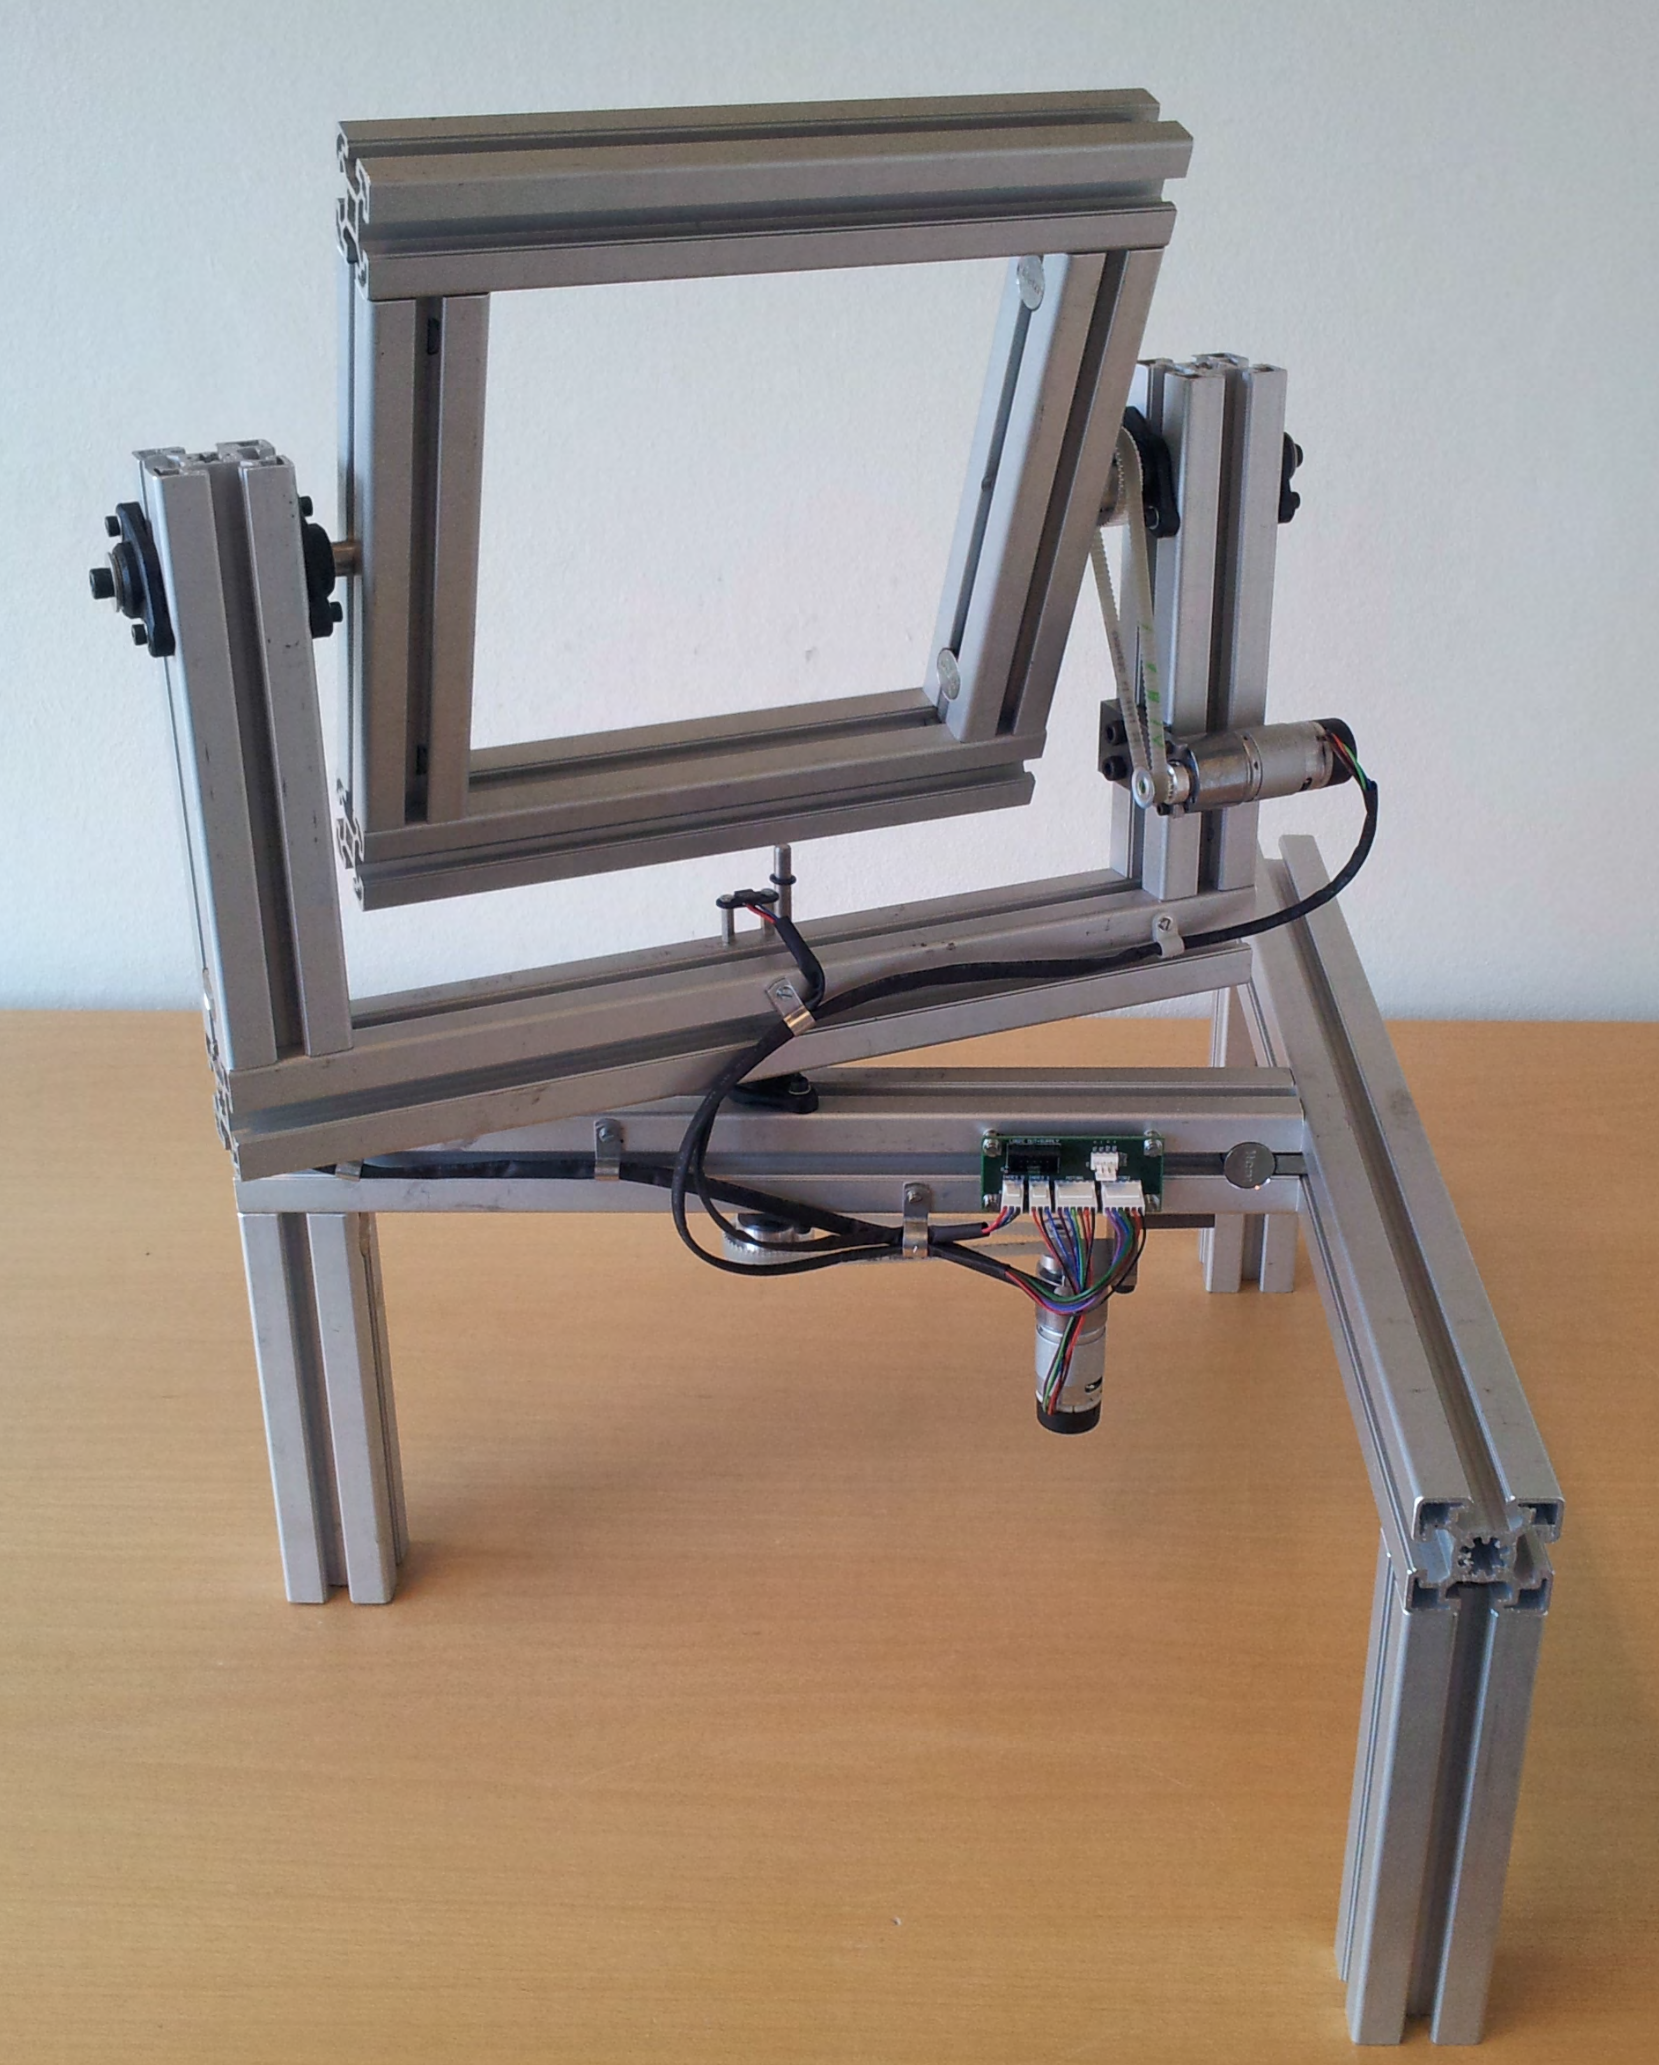
\includegraphics[width=0.5\textwidth]{\main/afsnit/introduction/images/pantilt.png}
\caption{Pan-Tilt system}
\label{fig:system}
\end{figure}

The use case, defined by the projectgroup, is mounting a stage lamp onto the system for use in theater or similar setting.
The angle of the light is controlled on both the pan and tilt axis through an interface with the Tiva microcontroller, either using the UART connection or the hardware input devices directly attached, these devices can be seen in figure \ref{fig:empboard}

\begin{figure}[H]
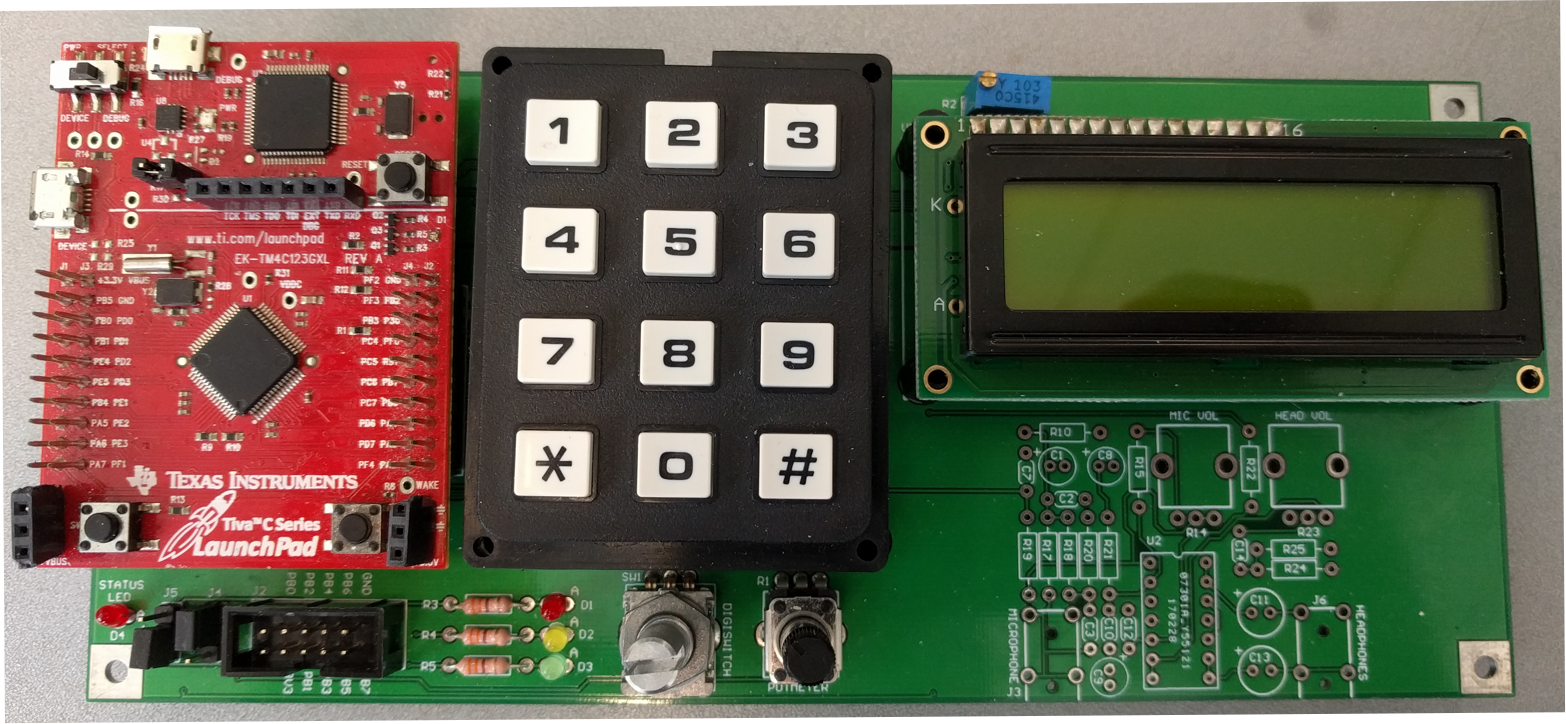
\includegraphics[width=\textwidth]{\main/afsnit/introduction/images/empboard.png}
\caption{EMP board provided to the project}
\label{fig:empboard}
\end{figure}

The use case is exclusively theoretical and aims to set the requirements for the system.
The pan tilt system is provided assembled and requires no further physical alterations. The scope of the project is therefore limited to software and control engineering decisions required to achieve a conforming, to set requirements, pan-tilt system for a stage lamp.

The project will be run on a  TM4C123GH6PM MCU installed on a TM4C123G LaunchPad Evaluation Kit made by Texas Instruments and a Artix-7 FPGA\footnote{Field Programmable Gate Array}. Software must be designed and written to allow these devices, in tandem to control the pan-tilt system, to move in a coordinated fashion.
The Tiva microcontroller will have software written in C while the FPGA behavior is defined using VHDL. The Tiva will control most of the logic of the system while the FPGA acts mainly as a hardware controller and data acquisition device.

\end{document}
